% mnras_template.tex
%
% LaTeX template for creating an MNRAS paper
%
% v3.0 released 14 May 2015
% (version numbers match those of mnras.cls)
%
% Copyright (C) Royal Astronomical Society 2015
% Authors:
% Keith T. Smith (Royal Astronomical Society)

% Change log
%
% v3.0 May 2015
%    Renamed to match the new package name
%    Version number matches mnras.cls
%    A few minor tweaks to wording
% v1.0 September 2013
%    Beta testing only - never publicly released
%    First version: a simple (ish) template for creating an MNRAS paper

%%%%%%%%%%%%%%%%%%%%%%%%%%%%%%%%%%%%%%%%%%%%%%%%%%
% Basic setup. Most papers should leave these options alone.
\documentclass[a4paper,fleqn,usenatbib]{mnras}

% MNRAS is set in Times font. If you don't have this installed (most LaTeX
% installations will be fine) or prefer the old Computer Modern fonts, comment
% out the following line
\usepackage{newtxtext,newtxmath}
% Depending on your LaTeX fonts installation, you might get better results with one of these:
%\usepackage{mathptmx}
%\usepackage{txfonts}

% Use vector fonts, so it zooms properly in on-screen viewing software
% Don't change these lines unless you know what you are doing
\usepackage[T1]{fontenc}
\usepackage{ae,aecompl}

%%%%% AUTHORS - PLACE YOUR OWN PACKAGES HERE %%%%%

% Only include extra packages if you really need them. Common packages are:
\usepackage{graphicx}	% Including figure files
\usepackage{amsmath}	% Advanced maths commands
\usepackage{amssymb}	% Extra maths symbols
\usepackage[xindy]{glossaries}
\glsdisablehyper
\usepackage{subcaption}
\captionsetup{compatibility=false}

%%%%%%%%%%%%%%%%%%%%%%%%%%%%%%%%%%%%%%%%%%%%%%%%%%

%%%%% AUTHORS - PLACE YOUR OWN COMMANDS HERE %%%%%

% Please keep new commands to a minimum, and use \newcommand not \def to avoid
% overwriting existing commands. Example:
%\newcommand{\pcm}{\,cm$^{-2}$}	% per cm-squared

\newcommand{\GSF}[1]{\noindent\textcolor{blue}{GSF:#1}}

\makeglossaries

%glossary
\newacronym{alfa}{ALFA}{Arecibo L-Band Feed Array}
\newacronym{dm}{DM}{Dispersion Measure}
\newacronym{frb}{FRB}{Fast Radio Burst}
\newacronym{fwhm}{FWHM}{Full-Width at Half-Maximum}
\newacronym{gbt}{GBT}{Greenbank Telescope}
\newacronym{htru}{HTRU}{High Time Resolution Universe}
\newacronym{igm}{IGM}{Intergalactic Medium}
\newacronym{ism}{ISM}{Interstellar Medium}
\newacronym{nip}{NIP}{Non-image Processing}
\newacronym{paf}{PAF}{Phased-Array Feeds}
\newacronym{rfi}{RFI}{Radio-frequency Interference}
\newacronym{ska}{SKA}{Square Kilometre Array}
\newacronym{sefd}{SEFD}{System Equivalent Flux Density}
\newacronym{snr}{SNR}{Signal-to-Noise Ratio}
\newacronym{sps}{SPS}{Single Pulse Search}
\newacronym{vlbi}{VLBI}{Very Long Baseline Interferometry}

%%%%%%%%%%%%%%%%%%%%%%%%%%%%%%%%%%%%%%%%%%%%%%%%%%

\title[The ALFABURST Commensal FRB Survey]{ALFABURST: A commensal search for
Fast Radio Bursts with Arecibo}

\author[G. Foster et al.]{Griffin Foster$^{1,2}$\thanks{E-mail: griffin.foster@physics.ox.ac.uk},
Aris Karastergiou$^{1,3,4}$,
Dan Werthimer$^{2}$,
\and Jayanth Chennamangalam$^{1}$,
Kaustubh Rajwade$^{5}$,
Golnoosh Golpayegani$^{6,7}$,
\and Duncan Lorimer$^{6,7}$,
Mayuresh Surnis$^{6,7}$,
Xin Pei$^{8}$
\\
% List of institutions
$^{1}$University of Oxford, Sub-Department of Astrophysics, Denys Wilkinson Building, Keble Road, Oxford, OX1 3RH, United Kingdom\\
$^{2}$Department of Astronomy, University of California, Berkeley, 501 Campbell Hall \#3411, Berkeley, CA, 94720, USA\\
$^{3}$Physics Department, University of the Western Cape, Cape Town 7535, South Africa\\
$^{4}$Department of Physics and Electronics, Rhodes University, PO Box 94, Grahamstown 6140, South Africa\\
$^{5}$Jodrell Bank Centre for Astrophysics, University of Manchester, Oxford Road, Manchester M13 9PL, United Kingdom\\ 
$^{6}$Department of Physics and Astronomy, West Virginia University, Morgantown, WV 26505, USA\\
$^{7}$Center for Gravitational Waves and Cosmology, West Virginia University, Chestnut Ridge Research Building, Morgantown, WV 26505, USA\\
$^{8}$Xinjiang Astronomical Observatory, Chinese Academy of Sciences, Urumqi, Xinjiang 830011, China\\
}

% These dates will be filled out by the publisher
\date{Accepted XXX. Received YYY; in original form ZZZ}

% Enter the current year, for the copyright statements etc.
\pubyear{2017}
\hypersetup{draft}
% Don't change these lines
\begin{document}
\label{firstpage}
\pagerange{\pageref{firstpage}--\pageref{lastpage}}
\maketitle

% Abstract of the paper
\begin{abstract}
% What is the point of the paper?
% What is the context of the study? What background information is necessary to understand the study?
% How was the study done?
% What is the main take away message?
% What can be said about these results, and how does this affect future work?
The ALFABURST fast radio burst (FRB) survey has been observing commensally with
other projects using the Arecibo L-band Feed Array (ALFA) receiver at the
Arecibo Observatory since July 2015. We report on the non-detection of any FRBs
from that time until August 2017 for a total observing time of 518 hours.  With
current FRB rate models, we expected to see multiple **how many??** FRBs based
on the total observing time, telescope sensitivity and beam size. We discuss the
implications of this non-detection of FRBs in the context of recent detections
with other telescopes and the limitation of our search pipeline.  During the
survey, single pulses from 17 known pulsars were detected.  We also report the
discovery of an interesting Galactic radio transient with a DM of 281
pc~cm$^{-3}$, which was detected while the telescope was slewing between fields.
\end{abstract}

% Select between one and six entries from the list of approved keywords.
% Don't make up new ones.
\begin{keywords}
radio continuum: transients -- methods: observational
\end{keywords}

%%%%%%%%%%%%%%%%%%%%%%%%%%%%%%%%%%%%%%%%%%%%%%%%%%

\section{Introduction}
\label{sec:intro}

\glspl{frb} are short-duration, broad-band, dispersed pulses that are detected
at radio frequencies. They are mostly classified by virtue of their dispersion
being far in excess of the expected Galactic contribution. As for radio pulsars,
for FRBs, where we observe the pulse over a frequency band ranging from $\nu_1$
to $\nu_2$, the resulting dispersion delay 
%
\begin{equation}
\Delta t \propto {\rm DM} \, (\nu_1^{-2} - \nu_2^{-2}),
\end{equation}
%
where the dispersion measure, DM, is the line integral of the electron column
density along the line of sight to the source.

Although the physical process that gives rise to FRBs is unknown, the
possibility that they originate at cosmological distances, and their potential
use as natural probes of large-scale structure and magnetoionic content of the
Universe makes them worthy of attention. They appear as bright sources at
telescopes on Earth, which indicates high luminosities given the implied
distance.  As short duration bursts, probably emanating from point-like sources,
they offer the unique opportunities to probe the inter-galactic medium (IGM)
\citep{2013ApJ...776..125M}, as pulsars do for the Galactic interstellar medium.

Since the first reported detection \citep{2007Sci...318..777L}, a number of
surveys using a range of radio telescopes have attempted to detect further
pulses. At the time of writing, 24 \glspl{frb} have been reported \citep[for an
up-to-date list, see][]{2016PASA...33...45P}. While the majority of these have
been detected with the Parkes Radio Telescope at 1.4~GHz (L-band), other
telescopes are making important contributions. FRB~121102 was detected in the
Pulsar Arecibo L-band Feed Array (PALFA) \citep{2014ApJ...790..101S}. This
\gls{frb} is the only known \gls{frb} to repeat \citep{2016ApJ...833..177S}.
FRB~110523 was detected with the Green Bank Radio Telescope (GBT) at 820~MHz
frequencies, confirming \glspl{frb} are observable outside L-band
\citep{2015Natur.528..523M}.  Recently, a number of very bright \glspl{frb} has
been detected with UTMOST \citep{2017MNRAS.468.3746C,atel10697} and ASKAP
\citep{2017ApJ...841L..12B}.

%FRB121002, detected with High Time Resolution Universe (HTRU) high latitude
%survey, was the first detected FRB with a clear two-component profile, was
%challenging one-off high energy FRB emission models
%\citep{2016MNRAS.460L..30C}.

Even with the current small sample of FRBs population, it is clear that their
properties vary significantly. The measured \glspl{dm} range from
176~pc~cm$^{-3}$ (FRB~170827) to 2596 pc~cm$^{-3}$ (FRB~160102), with pulse
widths ranging from sub-ms (unresolved) to 21~ms, and apparent flux densities
covering four orders of magnitude. The sky distribution of these sources appears
skewed towards high Galactic latitudes \citep{2015MNRAS.451.3278M}.
% TODO: I am not sure I believe this statement! Or at the very least, it hides a lot
%of details. To first order, the sky distribution is isotropic.

% TODO: i don't like this opening sentence yet
Single dish telescopes have been essential to detection of \glspl{frb}, and
continue to be useful for population statistics.  But, these telescopes provide
limited localization.  The unknown detection position in the primary beam, and
one-off nature of most of the \glspl{frb} does also not allow precise
determination of the absolute flux density or the spectral index. Only the
repeater FRB~121102 has been localized using \gls{vlbi}
\citep{2017ApJ...834L...8M, 2017ApJ...834L...7T}. Localization is key to
understanding \glspl{frb}. This requires the use of interferometric arrays with
arc-second accuracy, such as MeerKAT, ASKAP, and the SKA. 

Apart from localization, \gls{frb} spectra offer important clues on the nature
of the emission process. Low frequency searches with LOFAR
\citep{2015MNRAS.452.1254K}, MWA \citep{2015AJ....150..199T}, and the GBT
\citep{2017arXiv170107457C} have reported non-detections.  No large surveys for
\glspl{frb} have been done above L-band frequencies. This is, in part, due to
the narrowing of beam size which limits sky coverage.
\cite{2017arXiv170507553L} ran a coordinated-in-time, multi-telescope campaign
of the repeater \gls{frb}.  They report non-detection of pulses at VHF, C-band,
Ku-band during periods of detected bursts in L-band and S-band. \cite{atel10675}
report detections of FRB121102 from 4-8 GHz (C-band). In summary, our current
understanding of \glspl{frb} spectra is limited, however they appear not to
follow the steep power law example of radio pulsars, and may even not be smooth
and continuous with frequency.

For single dish telescopes there is a trade-off of sensitivity for survey speed.
Large beams, while providing a large sky coverage, have been unsuccessful at
detecting \glspl{frb}. Conversely, Arecibo provides the highest sensitivity, but
with a very narrow beam. Parkes appears to be near the optimal trade-off point
between sensitivity and beam size for this class of object. ASKAP dishes with
\glspl{paf} provide a large sky coverage with a significant enough sensitivity
to detect bright \glspl{frb}. Interferometric arrays such as CHIME and MeerKAT
while provide both sensitivity and sky coverage. One important question relating
to the nature of the \gls{frb} population is what are the statistics of source
numbers versus source flux density, and whether or not the cumulative flux
density distribution is consistent with a population of cosmologically
distributed standard candles. To answer this question, it is particularly
interesting to sample both extreme ends of the flux density axis: the brightest
\glspl{frb} discovered using small telescopes in long duration and large
sky-coverage surveys, as well as the weakest \glspl{frb} sampled through
high-sensitivity observations with large telescopes, necessarily sacrificing
survey time and sky coverage. 

In this paper, we describe a new experiment, ALFABURST, which has enabled high
sensitivity observations to better sample the low flux density end of the
population. ALFABURST makes use of the large amount of time spent by the ALFA
receiver for other astronomical surveys. The plan for the rest of this paper is
as follows. In Section \ref{sec:overview}, we summarize the survey parameters
and observations carried out so far.  A wide-feature, learned model was used to
classify each dataset in order to filter out radio-frequency interference and
create a priority queue for visual examination. This model and the
post-processing procedures are discussed in Section \ref{sec:event_classify}.
Although no FRBs have been found in observations carried out so far, we did
detect one pulse that is consistent with an origin in the Galactic plane. This
source is discussed in Section \ref{sec:18062017}. We discuss the expected event
rates in Section \ref{sec:event_rates}. Finally, in Section \ref{sec:discuss},
we consider possible explanations for our non-detection of FRBs so far and
speculate on future developments.

\section{Observations}
\label{sec:overview}

\subsection{ALFABURST description}

ALFABURST is an \gls{frb} search instrument which has been used to commensally
observe since July 2015 with other \gls{alfa} observations at the Arecibo
Observatory. This system is a component of the SETIBURST back-end
\citep{2017ApJS..228...21C} and uses ARTEMIS \citep{2015MNRAS.452.1254K} for
automated, real-time pulse detection. We perform inline radio-frequency
interference (RFI) removal, baselining using zero-DM removal
\citep{2009MNRAS.395..410E}, and spectrum normalization before single pulse
detection. During this time period a \gls{sps} was performed from \gls{dm} 0 to
10000, pulse widths from $256~\mu s$ to $16$~ms, across a 56~MHz bandwidth for
all 7 beams. We return to the effective \gls{dm} of the search in Section
\ref{sec:event_rates}. The gain of Arecibo allows for the most sensitive
\gls{frb} search to date.

Detections above a peak S/N of 10 were recorded along with an $8.4$~s dynamic
spectrum window around the event. When multiple events were detected in the same
time window, these events were pooled together and recorded to disk.
Approximately $2 \times 10^5$ 8.4~s datasets were recorded between July 2015 and
August 2017, the vast majority of which are false detections due to \gls{rfi}
signals passing the real-time \gls{rfi} exciser. We have detected no \glspl{frb}
in our commensal survey.

%%% SYSTEM VERIFICATION BEGINS %%%

\subsection{Single Pulse Search Verification}
\label{sec:system_verify}

PALFA survey scheduling includes regularly observing known pulsars to verify
timing analysis, this provides a consistent verification of our \gls{sps} to
detect pulses. As the PALFA survey is targeted at the Galactic plane a number of
high \gls{dm} pulsars were observed, single pulses from B1859+03 (\gls{dm}:
402), B1900+01 (\gls{dm}: 245) (Figure \ref{fig:B1900}), B2002+32 (\gls{dm}:
234), B1933+16 (\gls{dm}: 158), among others were detected.

% TODO: table of detected pulsars: max SNR, SNR-maximized DM, number of pulses

% alfaburst-initial-survey/notebooks/B1900_01.ipynb
\begin{figure}
    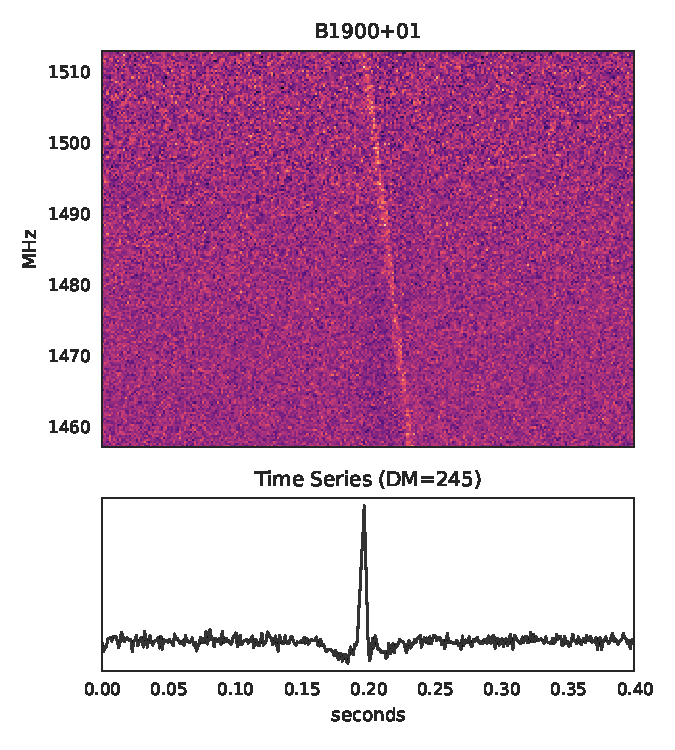
\includegraphics[width=1.0\linewidth]{figures/B1900_01.pdf}
    \caption{Detection of a single pulse from PSR B1900+01 (DM 245). The
    baseline dip before and after the pulse is due to zero-DM removal (Eatough
    et al.~2009). }
    \label{fig:B1900}
\end{figure}

%%% SYSTEM VERIFICATION ENDS   %%%

%%% SKY COVERAGE BEGINS %%%

\subsection{Survey Coverage}
\label{sec:survey_coverage}

Since ALFABURST was installed, the majority of ALFA observation time is
allocated for the AGES \citep{2006MNRAS.371.1617A} and PALFA
\citep{2006ApJ...637..446C} surveys (Figure \ref{fig:sky_coverage}).  The AGES
survey pointings are off the galactic plane, which is ideal for \gls{frb}
surveys.. PALFA is a pulsar search survey with pointings near the galactic
plane. These lines of sight can introduce significant dispersion due to the
\gls{ism}. We search out to a DM of 10$^{4}$~cm$^{-3}$~pc which is well beyond
the maximum Galactic dispersion, but within the technical capabilities of our
system. 

Approximately 65\% of the ALFABURST survey time has been in pointings out of the
galactic plane ($|b| > 5^{\circ}$).  These pointings are primarily from the
ongoing AGES survey.  Pointings in the plane are primarily from the PALFA
survey.  The PALFA survey detected the repeating \gls{frb} FRB121102
\citep{2014ApJ...790..101S}, the only \gls{frb} detected with Arecibo thus far.
As ALFABURST has been running commensally with the PALFA survey since 2015 these
two back-ends act as independent single-pulse search pipelines, useful for
detection verification.  Since the beginning of ALFABURST observations no
\glspl{frb} have been reported by PALFA. No follow-up observations of FRB~121102
have been conducted using ALFA.

% alfaburst-initial-survey/notebooks/Sky_Coverage.ipynb
\begin{figure*}
    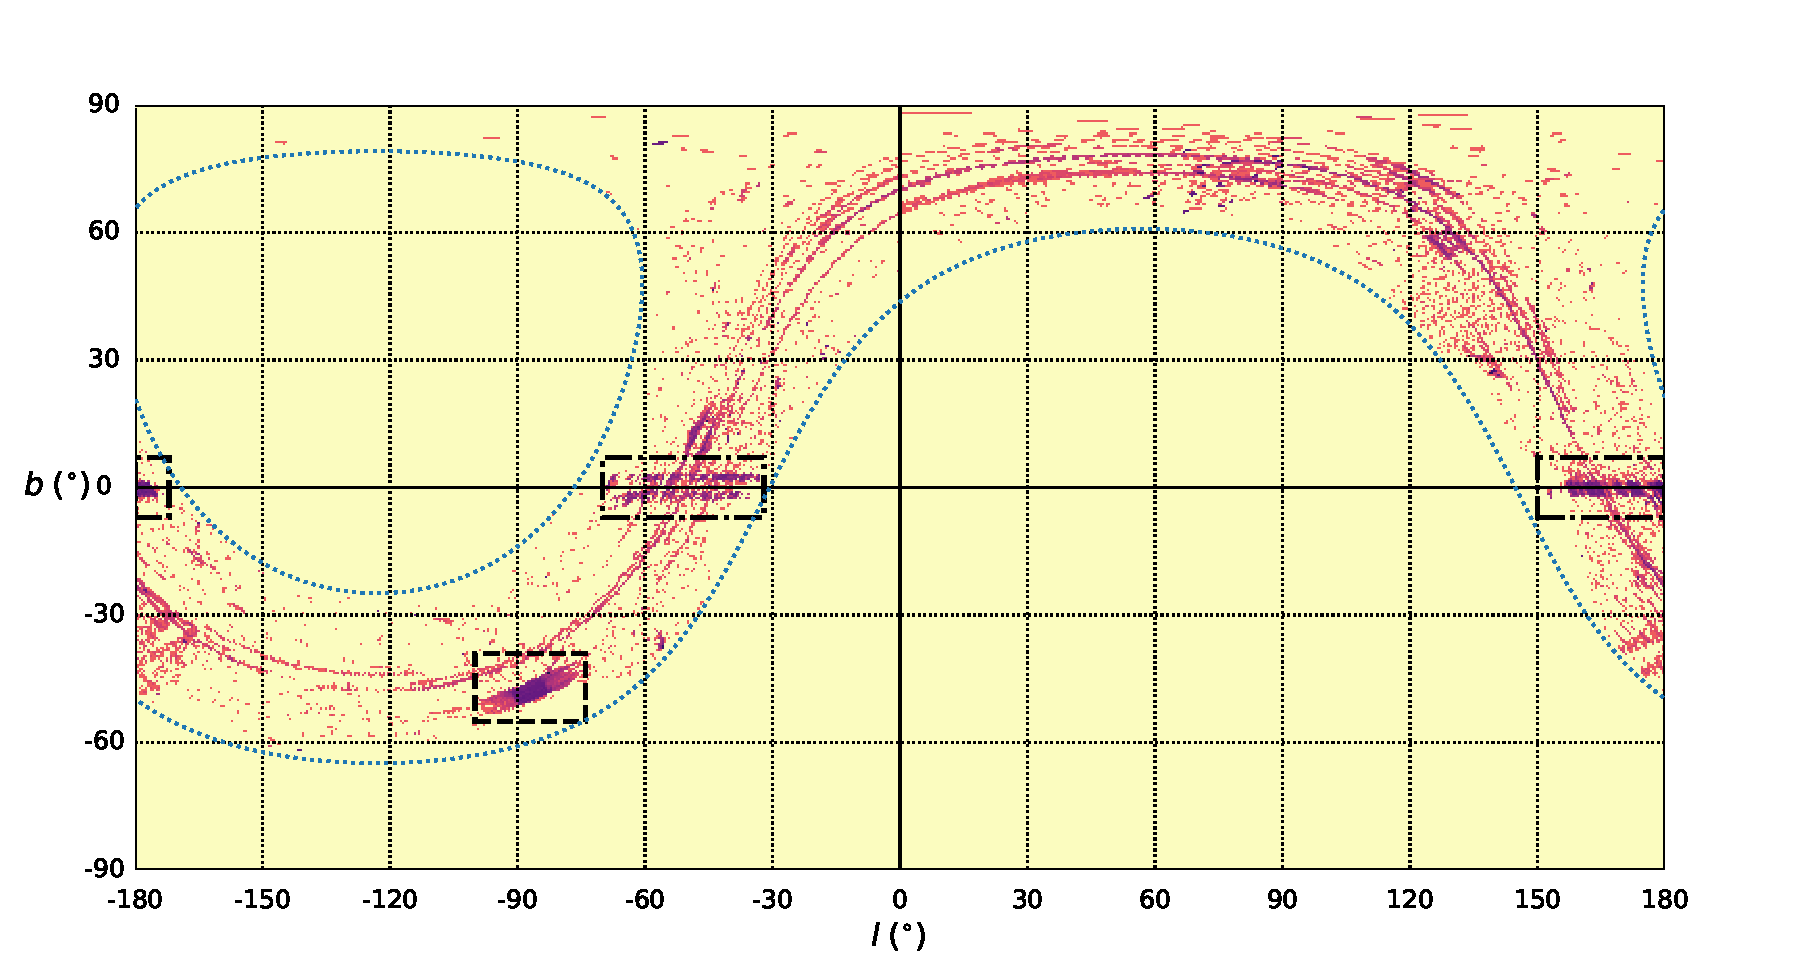
\includegraphics[width=1.0\linewidth]{figures/cartview_sky_coverage.pdf}
    \caption{Sky coverage during ALFA usage between July 2015 and June 2017,
    shown in a Cartesian projection in galactic coordinates along with
    declination pointing limits (blue dashed). Color represents total time
    pointing in a log scale. The majority of ALFA usage during this time was for
    the PALFA survey along the galactic plane (dot-dashed boxes) and the AGES
    survey (dashed box).  The S-shaped arcs across the plot are due to fixed
    pointings in local azimuth and altitude.
    }
    \label{fig:sky_coverage}
\end{figure*}

%%% SKY COVERAGE ENDS   %%%

%%% OBSERVATION TIME BEGINS %%%

\subsection{Observing Time}
\label{sec:obs_time}

From the beginning of July 2015 to the end of April 2017 \gls{alfa} has been
used for approximately 1400 hours of observing, with all seven beams functional.
Due to pipeline development and hardware reliability, ALFABURST was active and
functional for, on average, 322 hours per beam.  The current system is setup to
be reliably in use for all beams any time \gls{alfa} is active and in the
correct receiver turret position. Since April 2017 this stable version of the
pipeline has run for an additional 196 hours. This has resulted in a total of
518 hours of processed observing time since ALFABURST began commensal
observations.

%%% OBSERVATION TIME ENDS   %%%

%%% PRIORITIZER BEGINS %%%

\section{Event Classification Strategy}
\label{sec:event_classify}

% TODO:
% add figure
% ML references

The significant DM trial range, variety of \gls{rfi} events, and commensal
nature of the survey, leads to a large number of false detections. Approximately
$2 \times 10^5$ unique 8.4~s datasets were recorded with at least one detection
above the minimum peak signal-to-noise (S/N) threshold of 10. For each event
window, a diagnostic plot was generated which contained the original dynamic
spectrum, the dedispersed dynamic spectrum of the S/N-maximized DM, along with a
frequency collapsed time series of the detection. A set of statistics for each
of these plots was also computed when this figure was generated.

A sample of the datasets were labelled into 8 categories of RFI ***should we
expand on these 8 categories???***, systematic effects, and astrophysical source
(pulsars). Classification using these labels has not been constant throughout
the survey due to software improvement, and changes in telescope observing
strategy.

Pulses from known pulsars were used as a proxy category for the FRB class. The
number of astrophysical pulse detections was low compared to the number of
false-positive detections. It was necessary to use a large number of categories
as RFI and systematic effects took on a variety of forms.  This had the
additional effect of balancing out the number of events in each class, making
model training more robust.

These statistics along with the labels were used to build a random forest
probabilistic classifier model. All unlabelled datasets were given a probability
of belonging the predefined categories. In training the model we optimized for a
high recall, since in searching for \glspl{frb} we are inclined to allow for a
large number of false-positive events (detection due to RFI or systematics) as
long as there are no false-negative events (pulses classified as RFI).

Using a probabilistic multi-label classifier **reference to relevant papers?***
allows us to prioritize the order and amount of time we spend on examining event
datasets. Those with high probability of belonging to a single class can be
examined as a group quickly.  Datasets which fall into multiple classes are
examined more thoroughly, they are labelled by hand, and the set of features
extracted during the figure generation process is refined to further
differentiate classes. This model building, prioritizing, and examination
process was iterated on multiple times to improve the classifier. We continue to
iterate on this model and will use it for future prioritization of examining
events.

We have used our classifier model as a data exploration tool to add and refine
procedural filters to the data. We have not used the classifier model directly
in our pipeline as the black-box nature of the model can lead to
misclassification.  During the offline data examination process a number of
simple filters were developed to cut down on the number of false-positive
detections without relying on the classifier model. For example, datasets in
which the maximum DM of events was less than 50 were cut.  Given the optimal
dispersion measure, DM$_{\textrm{opt}}$, obtained from the S/N-maximized DM
trial,  if the DM range exceeds $(0.5 \times DM_{\textrm{opt}}, 1.5 \times
DM_{\textrm{opt}})$, then the event is due to long duration RFI and is cut.
Applying the various filters we reduced the number of datasets to approximately
30,000. The windows were sorted by S/N, and the top S/N events were examined
first.  During this process all datasets were labelled.  Astrophysical events
were identified based on the beam ID and pointing information.

%%% JUNE 18, 2017 BEGINS %%%

\section{The event of 2017, June 18}
\label{sec:18062017}

Though we report no detection of FRBs in the first two years of observations
with ALFABURST we have made an initial detection of an as yet unknown broad-band
(within our band) pulse (Figure \ref{fig:D20170618_spectrum}) at a peak S/N of
18. The peak S/N is maximized by dedispersion using a DM of 281~pc~cm$^{-3}$ and
time decimation factor 8. The pulse width is approximately 3 ms wide. The pulse
occurred in beam 5, and there were no other detections in the other beams at the
time.

% watermark:/home/griffin/data/alfa/D20170618/Beam5_fb_D20170618T005616.buffer2-paper.ipynb
\begin{figure}
    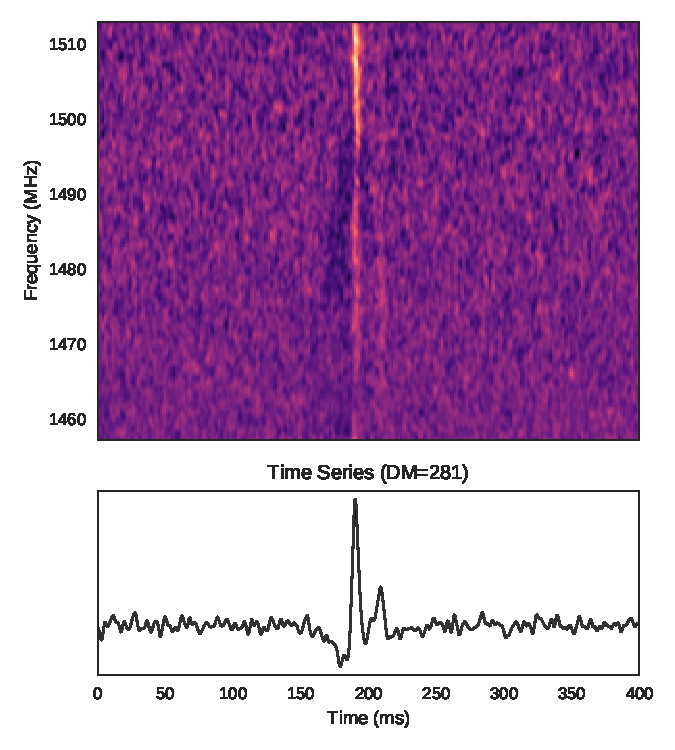
\includegraphics[width=1.0\linewidth]{figures/Beam5_fb_D20170618T005616_buffer2_spectrum.pdf}
    \caption{A broad band pulse (S/N maximized at DM~$=281$~pc~cm$^{-3}$)
    detected in beam 5 while the telescope was slewing during a PALFA
    observation. There is no known source which has been associated with this
    detection. As the observation was in the galactic plane it is likely
    galactic in origin.
    }
    \label{fig:D20170618_spectrum}
\end{figure}

The shape of the pulse is made up of two clear components, with the secondary
pulse arriving approximately 20 ms after the primary pulse, as seen in the
dynamic spectrum (Figure \ref{fig:D20170618_spectrum}). In DM-time space the
event is compact, consistent with a $\nu^{-2}$ dispersion relation (Figure
\ref{fig:D20170618_dmspace}), though such a fit has large error bars due to the
small fractional bandwidth that is processed with ALFABURST.

% watermark:/home/griffin/data/alfa/D20170618/Beam5_fb_D20170618T005616.buffer2-paper.ipynb
\begin{figure}
    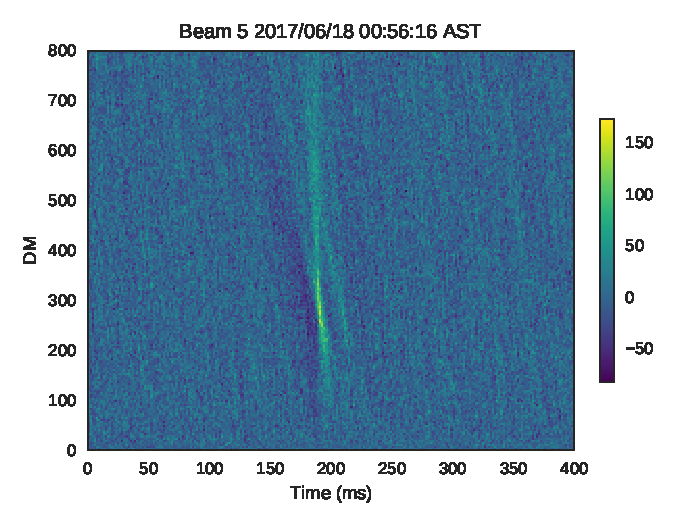
\includegraphics[width=1.0\linewidth]{figures/Beam5_fb_D20170618T005616_buffer2_dmspace.pdf}
    \caption{DM-time plot of the 2017 June 18 pulse. The pulse is compact in
    DM-time space, consistent with an astrophysical event. The secondary pulse
    20 ms after the primary pulse causes the intensity to be slightly elongated
    to higher trial DMs.
    }
    \label{fig:D20170618_dmspace}
\end{figure}

The detection occurred at 04:56:16 UT on 2017, June 18 (MJD 57922) during a
PALFA observing run. The event was not seen by the PALFA collaboration as it
occurred when the telescope was slewing between fields and the PALFA
spectrometers were not running. This is the first known detection of a
transient, broad-band pulse using ALFA during such a slew. However. this makes
it challenging to determine the accurate source position. Pointing information
from Arecibo is reported every second.  During the detection the pointing was
changing by approximately 5 arcminutes per second in right ascension 2
arcminutes per second in declination. This rate gives us a conservative estimate
of the error in pointing at the time the pulse was detected. Based on the time
stamp of the pulse and the pointing data the pulse occurred when beam 5 of ALFA
was pointing at right ascension: 18~h 45~$\pm 5$~m, and declination: +00 d
38'~$\pm 2$ (Galactic coordinates $l: 32.7812, ~b: +1.6850$).
% TODO: pointing error refinement

This beam 5 pointing is close to the Galactic plane in the first quadrant. The
DM distance estimated from the NE2001 model \citep{2002astro.ph..7156C} is
approximately 6 kpc, which is well within the Galaxy. The maximum Galactic
contribution along this line of sight would produce a DM of
$\sim800$~pm~cm$^{-3}$.  A search of the ATNF pulsar
database\footnote{http://www.atnf.csiro.au/people/pulsar/psrcat}
\citep{2005AJ....129.1993M}, RRAT
catalog\footnote{http://astro.phys.wvu.edu/rratalog}, and recent PALFA
discoveries \footnote{http://www.naic.edu/$\sim$palfa/newpulsars/} revealed no
known source with a DM near 281 pc~cm$^{-3}$ within a degree of the pointing.

As the telescope was slewing at the time, the source was only in the primary
lobe for a fraction of a second (assuming it was in the primary lobe and not a
side lobe).
% TODO: What is the maximum duration pulse that could be seen given the slew rate and beam size??
It could therefore be an RRAT which we
serendipitously detected at the correct moment, or it could be an individual
pulse from a pulsar. This region has been previously surveyed with PALFA and the
Parkes Multi-beam Survey \citep{2001MNRAS.328...17M} with no significant
detection of a pulsar at this DM.

The pulse appears brighter at higher frequencies, which could be due to
scintillation. Another reason for this frequency-dependent structure is that the
pointing of the telescope is changing during the total dispersion time of the
pulse within the observed band. As the pointing moves, the corresponding
telescope gain also changes.  There was a higher beam gain at the beginning of
the pulse compared to the end of the pulse, inducing a frequency-dependent gain
response due to the beam, also known as \emph{spectral colorization}.  A more
detailed analysis of this event, which will include follow-up observations, will
be presented elsewhere.

%%% JUNE 18, 2017 ENDS %%%

%%% EVENT RATES BEGINS %%%

\section{Expected FRB Events}
\label{sec:event_rates}

The currently known 24 FRBs vary significantly in \gls{dm}, pulse
width, and flux density. Despite this, we assume a simple model to
derive an expected event rate with our survey.  We use a model
\citep{2013MNRAS.436L...5L} which assumes \gls{frb} sources are
standard candles with a fixed spectral index, uniformly distributed in
co-moving volume. The event rates in this model are scaled to the
event rates reported in \cite{2013Sci...341...53T}. 
% TODO: Why are we using such an old event rate???

Taking advantage of the large forward gain of Arecibo, we account for
the sensitivity of the 7 ALFA beams out to outer edge of the first
sidelobe. In practice we do this by splitting the beam and first
sidelobe into shells of progressively lower gain but larger sky
coverage, and integrate to obtain the totals.

An \gls{alfa} beam is approximately 3.8'~$\times$~3.3' at \gls{fwhm} across the
band.  The ALFA beam size is known to be relatively fixed in size across the
band due to the optics \citep{GALFAbeam}.  Given the average observing time per
beam of 518 hours this results in a survey coverage of $\sim 10 \;
\textrm{deg}^2 \; \textrm{hours}$ when accounting for all 7 beams. This is a
small survey coverage compared to most other \gls{frb} surveys, primarily due to
the narrow beam size of Arecibo. The combined Parkes multi-beam surveys have a
total of 8231 observation hours \citep{2016MNRAS.460.3370C}, and a FWHM survey
metric of $\sim 4500 \; \textrm{deg}^2$ hours.  ALFABURST does not compete with
other surveys on sky coverage, rather it competes on sensitivity.  Using
Equation 6 of \cite{2015MNRAS.452.1254K}, a  single-pulse-search pipeline is
sensitive to pulses with a minimum flux density
%
\begin{equation}
S_{\rm min} = \textrm{SEFD} \frac{\textrm{S/N}_{\rm min}}{\sqrt{D \; \Delta \tau \;
\Delta \nu}}
\end{equation}
%
which is a function of the telescope \gls{sefd}, the minimum S/N
detection level $\textrm{S/N}_{\rm min}$ and the decimation rate $D$
compared to the native instrumental time resolution $\tau$, this comes
from the search pipeline which averages together spectra to search for
scattered pulses. ALFABURST has a native resolution of $\Delta \tau =
256 \; \mu s$, effective bandwidth $\Delta \nu = 56 \textrm{MHz}$, and
$\textrm{S/N}_{min} = 10$. The FWHM \gls{sefd} of the \gls{alfa}
receiver is approximately 3 Jy across the band for all beams.

The \gls{sps} pipeline is configured to search for pulses from 256~$\mu$s to 16
ms. Considering only the main beam lobe, a perfect matched filter would result
in a sensitivity to pulses with a minimum flux of $S_{256 \mu\textrm{s}} = 250$
mJy to $S_{16 \; \textrm{ms}} = 31$ mJy \citep{2015MNRAS.452.1254K}. Figure
\ref{fig:fwhm_sefd_z} shows the peak flux density of using the standard candle
\gls{frb} model as a function of source redshift for different model spectral
indices. The dashed lines of constant flux show the sensitivity of the ALFABURST
search pipeline to pulses of different widths. Assuming a positive spectral
index model ($\alpha=1.4$) results in a sensitivity out to the maximum
redshift/\gls{dm} for pulses with widths of at least 1 ms. A flat spectral index
model results in sensitivity from $z \sim 1.5$ (256~$\mu$s) out to $z \sim 5$
(16~ms) depending on pulse width. A negative spectral index model ($\alpha \sim
-1.4$) limits the survey to $z < 3$ for all pulse widths.

% alfaburst-initial-survey/notebooks/ALFABURST_Derived_FRB_Rates.ipynb
\begin{figure}
    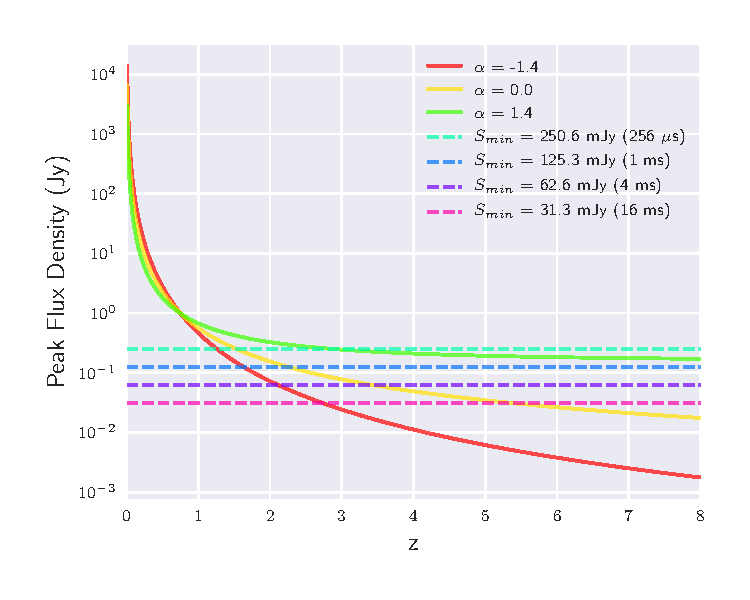
\includegraphics[width=1.0\linewidth]{figures/fwhm_sefd_z_relation.pdf}
    \caption{Sensitivity of the ALFABURST search pipeline (dashed) to FRB pulses
    assuming a standard candle model using different spectral index models
    (solid).
    }
    \label{fig:fwhm_sefd_z}
\end{figure}

If we assume a simple model of $\alpha=0$ as we have limited information about
the source spectral index, and a pulse width of 4 ms as that is an approximate
median pulse width of reported \glspl{frb}, then this results in a maximum
redshift of $z=3.4$ (a co-moving distance of 6.8 Gpc) and a survey volume of $6
\times 10^5$ Mpc$^3$ when using all 7 \gls{alfa} beams. The number of galaxies
sampled in this volume is $6 \times 10^3$ assuming a constant galaxy number
density of $10^{-2}$ per Mpc$^3$.  The volumetric event rate from
\cite{2013Sci...341...53T} is stated to be $R_{\textrm{FRB}} = 10^{-3}$
\glspl{frb} per galaxy per year. With these assumptions, we should expect to
detect $\sim 1$ \glspl{frb} based on the current observation time. We note once
again that the areal covereage used in this calculation is only based on the
sensitivity and size of the main beam lobe.

% TODO:
% One thing that I think is needed here is to move to more recent rate
% estimates. If we go to something like Rane et al --- then that's at least a
% factor of two less than Thornton et al, with a range something like 1000--9000
% FRBs per day per sky out to redshift of one. I think if we just put the event
% rate range into these estimates then the above calculation will move from $\sim
% 1$~FRB o $<1$~FRB and there will not necessarily be any conflict with a
% non-detection.

As mentioned above, it is worth also taking into account the entire
first side lobes of the beams as Arecibo would be sensitive to detect
most previous \glspl{frb} in these. Using the parameterized \gls{alfa}
beam model (Figure \ref{fig:alfa_beam}) \citep{GALFAbeam} we can
compute the \gls{frb} survey metric and expected rates as a function
of beam sensitivity.  The first side lobes peak at around $-10$ dB and
provide a significant increase in sky coverage compared to just the
primary lobes.

% alfaburst-initial-survey/notebooks/ALFABURST_Derived_FRB_Rates.ipynb
\begin{figure}
    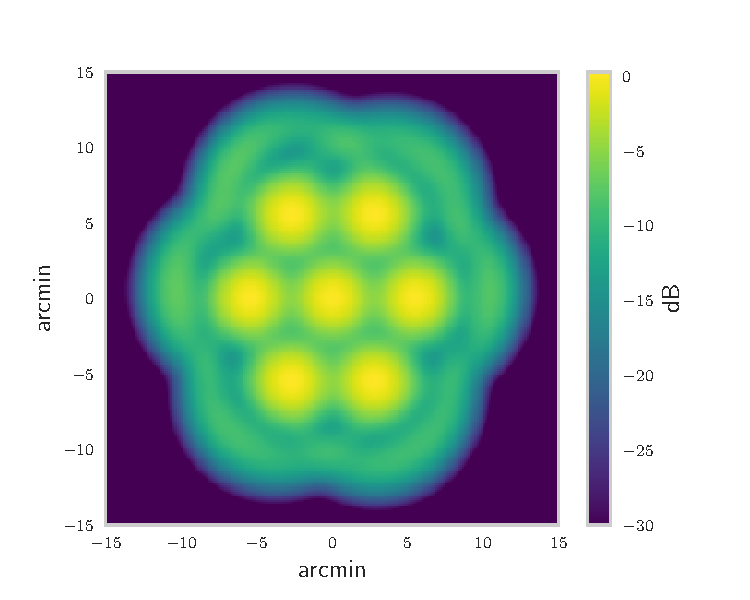
\includegraphics[width=1.0\linewidth]{figures/ALFA_beam_1425MHz_dB.pdf}
    \caption{Primary and first side lobe model of the AFLA receiver in
    decibels, cut-off at $-30$ dB.The first side lobe peak at around $-9$ dB.
    }
    \label{fig:alfa_beam}
\end{figure}

The total survey metric can be computed as a function of the beam
sensitivity by integrating over the beam (Figure
\ref{fig:survey_metric_sense}). We convert the beam model to units of
Jy by assuming that the $-3$ dB point corresponds to the \gls{fwhm}
SEFD of 3~Jy. The survey metric increases to approximately $30 \;
\textrm{deg}^2$ hours by including more of the primary beam beyond the
\gls{fwhm} point. The steep further increase in the survey metric seen
in Figure \ref{fig:survey_metric_sense} arises from including the
first side lobes. The long tail comes from the residual sensitivity by
integrating over the remaining beam.

% alfaburst-initial-survey/notebooks/ALFABURST_Derived_FRB_Rates.ipynb
\begin{figure}
    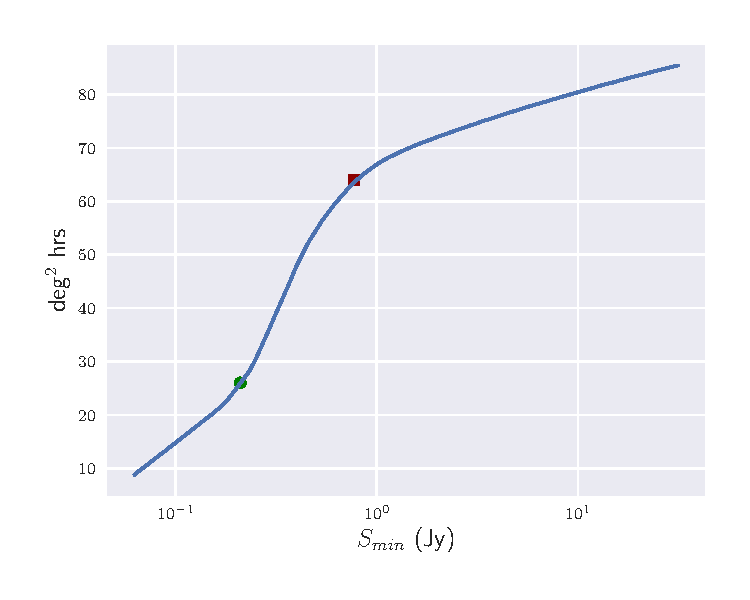
\includegraphics[width=1.0\linewidth]{figures/full_survey_metric_sense.pdf}
    \caption{Survey metric as a function of the ALFA receiver minimum
    sensitivity using the ALFA primary and first side lobes. The $-9$ dB point
    (green circle) which is the beginning of the first side lobe sensitivity and
    $-12$ dB point (red square) which is the FWHM of the first side lobe are
    marked.
    }
    \label{fig:survey_metric_sense}
\end{figure}

The survey volume is significantly increased by including a large
portion of the beam. It is not possible to put together a figure
similar to Figure \ref{fig:fwhm_sefd_z} when considering the full
beam. It is however possible, under the assumption of flat intrinsic
FRB spectra, to compute the maximum redshift as a function of beam
size and sensitivity. Plotting the survey metric as a function of
maximum redshift (Figure \ref{fig:full_sefd_z}) shows how the full
beam model increases the survey metric as a function of redshift. The
total survey volume is computed by integrating over redshift.
Including additional ALFA side lobes results in minimal increase in
the survey volume.

% alfaburst-initial-survey/notebooks/ALFABURST_Derived_FRB_Rates.ipynb
\begin{figure}
    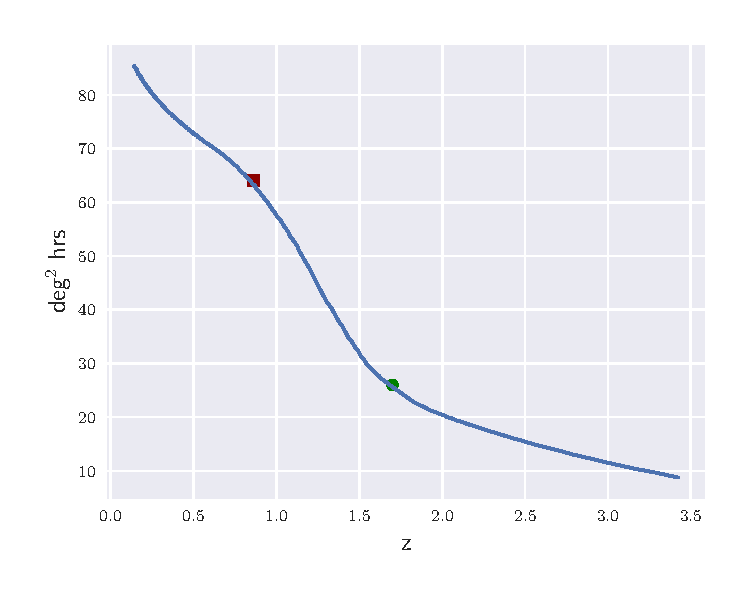
\includegraphics[width=1.0\linewidth]{figures/full_sefd_z_relation.pdf}
    \caption{Survey metric as a function of redshift using the standard candle
    model with a flat spectral index ($\alpha=0$) and pulse width of 4 ms. The
    bump out to $z=1.5$ is due to the including the ALFA first side lobes.
    Markers indicate the $-9$ dB (green circle) and $-12$ dB (red square) of the
    ALFA beam.
    }
    \label{fig:full_sefd_z}
\end{figure}

The integrated survey volume out to the first side lobe is $5.8 \times
10^6$ Mpc$^3$. The expected number of \glspl{frb} in the survey is
$\sim 3$ when using the galaxy number density and $R_{\textrm{FRB}}$
stated above. Though this event rate is more complex to model, it
provides a more accurate assessment of the expected detection rates
based on the apparent flux of previously reported \glspl{frb}. We note
that the volume we are sampling is biased towards small distances, due
to the large sky coverage of the low sensitivity outer parts of the
beam.

% TODO: stopped here

** I suggest clearly adopting an all-sky event rate
with 95\% confidence interval and using that interval
to more robustly determine the expected number of FRBs.

In the analysis above, we have not provided error estimates to our
total expected events. We are assuming standard candle FRBs and flat
spectra, assumptions which are impossible to attribute error margins
to. The significance of our result is difficult to quantify, beyond
stating that, under reasonable assumptions and previous detections, we
would have expected an FRB in our survey. However, the non-detection
cannot be assumed to imply significant discrepancy with our current
understanding of this population.

% TODO: split apart
\subsection{Sensitivity Upper Limit}
\label{sec:upper_limit}

The sensitivity limit of ALFABURST is determined by the telescope
sensitivity and receiver beam model. However, there is also a
sensitivity upper limit due to the real-time parameterized \gls{rfi}
exciser. The choice of these parameters sets an upper limit on the
flux of a pulse before it a portion of the flux is clipped and
replaced. Individual frequency channels in a spectra are replaced when
they exceed a threshold $T_{\textrm{chan}}$ after the spectra is
normalized ($\mu=0$, $\sigma=1$). And, entire spectra are clipped when
the summed spectra exceeds a threshold $T_{\textrm{spectra}}$. For
standard ALFABURST operation $T_{\textrm{chan}} = 5$ and
$T_{\textrm{spectra}} = 10$.

For very bright, small \gls{dm} pulses the \gls{rfi} exciser will replace
channels or spectra, reducing the overall flux or potentially removing the
entire pulse.  For bright, high \gls{dm} pulses the spectra will likely not be
replaced, but individual channels may be, resulting in a lower detected flux.
The \gls{rfi} exciser only works in the undecimated-in-time case ($D=1$), that
is the sensitivity that we are most concerned about when setting the \gls{rfi}
exciser thresholds.

\glspl{frb} detected at L-Band range between 200 mJy to a few Jy in flux
density, typically on the order of 5-10 milliseconds. For the sensitivity of the
\gls{alfa} receiver, individual channels of flux greater than 2.8 Jy will be
flagged, this will not have an effect on our ability to detect even the
brightest \glspl{frb}.  The maximum integrated pulse flux ($256 \; \mu$s width,
\gls{dm} $=0$) is $\sim250$ mJy before the pulse is clipped. The maximum
detectable flux increases as the square-root of the pulse width.  We see in
verification observations of bright, low \gls{dm} pulsars that individual
pulses are often excised. But, as we are interested in detecting high \gls{dm}
\glspl{frb} we have a higher upper limit as the flux is spread over multiple
spectra.

For reference, the minimum \gls{dm} of a pulse before the at least one channel
is shifted to the next spectra in time is \gls{dm} $=1.8$ pc cm$^{-3}$ for the
typical ALFABURST observing band (using Eq. 5.1 of \cite{2004hpa..book.....L}).
And, the minimum \gls{dm} before each frequency channel is in a separate spectra
is \gls{dm} $=976$ pc cm$^{-3}$. Most reported \glspl{frb} fall with in this
\gls{dm} range, so we consider a test \gls{frb} with a dispersion measure of 250
pc cm$^{-3}$ and narrow pulse width of $256 \; \mu$s to report our survey
upper-limit sensitivity. A \gls{dm} of 250 pc cm$^{-3}$ results in approximately
$1/128$ of the pulse per spectra. A bright pulse ($>32$ Jy) would be excised as
\gls{rfi} in this test case. This an extreme case, as most \glspl{frb} are wider
in width and at higher \glspl{dm}.  Our pipeline would preserve the flux of all
detected \glspl{frb} except the extreme FRB150807, and possibly FRB170827
(Figure \ref{fig:sensitivity_range}).  This also assumes the \gls{frb} is
detected at boresight, we would still be sensitive to such bright pulses in the
side lobes.

Figure \ref{fig:sensitivity_range} shows that ALFABURST sensitivity region based
on pulse width and peak flux, assuming detection at boresight. The ALFABURST
sensitivity region (purple) indicates the survey would be able to detect the
vast majority of previously reported \glspl{frb}. The upper flux limit cut-off
due to \gls{rfi} mitigation would have clipped out some flux from the extremely
bright, narrow, and low-DM FRB150807. Though, a portion of the flux would have
remained, and the \gls{frb} would have still been detected as significant.
Recent detections with UTMOST \citep{2017MNRAS.468.3746C,atel10697} indicate
that the parameter space in pulse width should be extended.  FRB160317 has a
measured pulse width of 21 ms. Currently the pipeline decimates in time out to
16 ms. The pipeline still sensitive to wider pulses, but at a loss in S/N
as indicated in the slight slope on the right side of the purple region of
Figure \ref{fig:sensitivity_range}, but we would not have detected FRB160317. It
is a minor change to our pipeline to increase the maximum pulse-width search.

% alfaburst-initial-survey/notebooks/Fluence_Rate.ipynb
\begin{figure}
    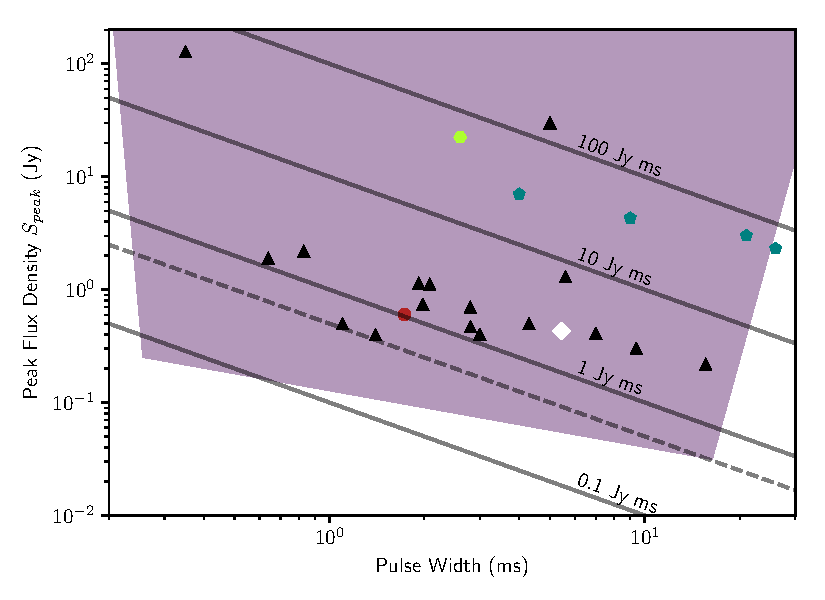
\includegraphics[width=1.0\linewidth]{figures/sensitivity_range.pdf}
    \caption{ALFABURST single pulse sensitivity (purple region). Automated RFI
    excision excludes narrow in width, low DM, bright FRBs such as FRB150807
    (yellow region).  Previously detected FRBs from Parkes (black triangle), GBT
    (red circle), Arecibo (white diamond), UTMOST (teal pentagon), and ASKAP
    (yellow-green hexagon) are plotted for reference. Line of constant fluence
    (solid) are plotted for reference. The fluence completeness (dashed) is 0.5
    Jy ms out to pulse widths of 16 milliseconds.
    }
    \label{fig:sensitivity_range}
\end{figure}

%%% EVENT RATES ENDS   %%%

%%% FLUENCE RATE BEGINS %%%

%\subsection{Fluence Completeness}
%\label{sec:fluence}

The fluence completeness of the survey \citep{2015MNRAS.447.2852K} is determined
by the minimum detectable fluence at the maximum sampled pulse width in the
survey. ALFABURST has a fluence completeness of $0.5$ Jy ms up to a pulse width
of 16 ms (Figure \ref{fig:sensitivity_range}). All previously reported FRBs are
within this completeness sample except for those noted in Section
\ref{sec:upper_limit}.

%%% FLUENCE RATE ENDS   %%%

\section{Discussion}
\label{sec:discuss}

Multiple factors could be contributing to our non-detection with the ALFABURST
survey. We derived an expected event rate based on the telescope sensitivity,
observing time, and a standard candle model \citep{2013MNRAS.436L...5L}. This is
a simple model based on the empirical event rates from detections in the
\gls{htru} survey \citep{2013Sci...341...53T}. The repeating nature of
FRB121102 indicates that there could be multiple classes of \gls{frb}
progenitors, or this standard candle model does not accurately model event
rates. The detection of bright, high-DM \glspl{frb} with ASKAP
\citep{2017ApJ...841L..12B} and UTMOST \citep{2017MNRAS.468.3746C,atel10697}
might indicate that \glspl{frb} are not standard candles.

The limited processing bandwidth of ALFABURST may be a cause of the survey
non-detection. Multiple detected \glspl{frb} show apparent scintillation and
steep spectral indices. It is not possible to differentiate between an apparent
spectral index induced by the beam or an absolute spectral index from the
source. Though, the localization and repeated detections of FRB121102 show there
is significant spectral variation from the source or due to the intervening
medium. Other \glspl{frb} show frequency-dependent structure which could be due
to beam colorization, intrinsic structure, or due an intermediate effect. Plasma
lenses in the \gls{frb} progenitor host galaxy could be modulating the pulse
amplitude as a function of frequency and time (if the source repeats)
\citep{2017ApJ...842...35C}. This effect introduces an additional uncertainty in
the \gls{frb} rate modeling as the apparent spectral indices of detected
\glspl{frb} may not be intrinsic. Thus, the observed frequency structure in an
\gls{frb} (repeating or not) would be dependent on multiple factors including
observing frequency, bandwidth, epoch, and even sky direction. If an \gls{frb}
did occur in the field of view of the telescope while ALFABURST was in operation
we could have been unlucky and scintillation or lensing caused the pulse in the
band to go below the detection threshold. Assuming no scintillation or lensing,
an increase to the full \gls{alfa} band would result in a $\sqrt{6}$ increase in
sensitivity. But, also important is a more complete sampling of the frequency
space if these effects are modulating the pulse.

\cite{2015MNRAS.451.3278M} conclude that the apparent deficit of \glspl{frb} at
low galactic latitudes is due to diffractive interstellar scintillation. Their
model shows that the true event rate is a factor of $\sim 4$ lower than the rate
reported in \cite{2013Sci...341...53T}, which the rate used in the standard
candle model \citep{2013MNRAS.436L...5L}. Though the ALFABURST survey is evenly
split across high and low galactic latitudes.  \cite{2015MNRAS.451.3278M} predict
that the increase in sensitivity of using Arecibo compared to Parkes should
result in a factor of 14 increase in detections, assuming a similar bandwidth
($\sim 300$ MHz). Accounting for the smaller bandwidth of ALFABURST means there
should still be a factor of a few increase in rates. This non-detection result
indicates that the \cite{2015MNRAS.451.3278M} flux density distribution is not
as steep as predicted.

The sensitivity of Arecibo allows the ALFABURST survey to probe a search volume
out to higher red-shifts than other surveys. In the standard candle model a flat
luminosity function is assumed. If there is a peak similar to the star formation
rate around $z=2$ \citep{2014ARA&A..52..415M} than the expected event rate
should be lower. Similarly, if \glspl{frb} are intrinsically steep spectra then
distant \glspl{frb} will have a decreased observed flux at L-band, possibly
below the search sensitivity threshold. \cite{2017arXiv170507553L} report
FRB121102 to be band limited during simultaneous observation campaigns using
multiple telescopes to cover a broad range of the radio band. \cite{atel10675}
observed 15 pulses from FRB121102 across the 4-8 GHz band and reported spectral
variation over a brief period of time. A high redshift, band-limited \gls{frb},
which ALFABURST is sensitive to, could be shifted below L-band. Such a pulse
would not be detected with ALFABURST.

% Possible reasons for non-detection:
%   * standard candle model:
%   * scintillation:
%       * limited bandwidth, repeater band varies
%       * relation to Macquart and Johnston paper: rate off/on the plane is
%       different due to scintillation regimes
%       * Macquart and Johnston: discount scintillation effects, they make predictions that
%       a number of FRBs should be detected with Arecibo. Our non-detection refutes this.
%       * repeater and low freq frb searches: spectra are not pulsar like. may be
%       due to strong scintillation
%   * plasma lens model (cordes et al.):
%       * narrow bandwidth
%   * Star formation rate:
%       * implied FRB Luminosity function: cosmological star formation rate, peaks
%       around z=2, Madau & Dickinson 2014
%   * steep spectrum/band limited:
%       * Law et al see no detections at low and 5 GHz+ freqs -> band limited,
%       steep spectrum ; we are probing a large z, perhaps the band is shifted
%       out of L-band
%       * FRB121102 shows dramatic frequency structure over wide bands

\section{Future Work}
\label{sec:future_work}

The ALFABURST system will continue to run commensally with other ALFA projects,
leading to an improvement on the event rate of low-fluence \glspl{frb}.  The
current \gls{sps} pipeline is undergoing a significant upgrade. The input
bandwidth is limited to 56 MHz of the full 336 MHz digital band due to IO
limitations. A new pipeline developed for \gls{ska} \gls{nip} will be used to
process the full \gls{alfa} band.  This will increase sensitivity, and improve
detection rates for scintillating or lensed \glspl{frb}.  An improved version of
the real-time \gls{rfi} exciser is currently being developed and will be
deployed to reduce the false detection rate. The post-processing classifier and
prioritizer model is being updated to make use of an auto-encoder to select deep
features and auto-generate classes. This will allow for an improved follow-up
and analysis cycle.

Over the time period ALFABURST has been active, the use of \gls{alfa} has
decreased as the PALFA and AGES surveys end. The 327 MHz and L-band wide feeds
are commonly used. We are generalizing the \gls{alfa} specific \gls{sps}
pipeline to be used when these feeds are active, increasing our survey time and
sampling a larger portion of frequency space. Additionally, our search pipeline
will be duplicated for use on the \gls{gbt} to be commensally run with L-band
observations. 

Jupyter notebooks are hosted on our public git
repository\footnote{https://github.com/griffinfoster/alfaburst-initial-survey}.

\bibliographystyle{mnras}
\bibliography{alfaburst.bib} 

\bsp	% typesetting comment
\label{lastpage}
\end{document}

% End of mnras_template.tex
